
% This LaTeX was auto-generated from an M-file by MATLAB.
% To make changes, update the M-file and republish this document.

\documentclass{article}
\usepackage{graphicx}
\usepackage{color}

\sloppy
\definecolor{lightgray}{gray}{0.5}
\setlength{\parindent}{0pt}

\begin{document}

    
    
\subsection*{Contents}

\begin{itemize}
\setlength{\itemsep}{-1ex}
   \item EEE 178 Homework \#4
   \item Problem 1
   \item Parts 1 and 2
   \item Part 3
   \item Part 4
   \item Part 5
   \item Part 6
   \item Problem 2
   \item Part 1
   \item Part 2
   \item Part 3
   \item Part 4
   \item Part 5
   \item Part 6
   \item Parts 7 and 8
   \item Problem 3
\end{itemize}


\subsection*{EEE 178 Homework \#4}

\begin{par}
MATLAB code and figures
\end{par} \vspace{1em}
\begin{verbatim}
clear all;
clc;
close all;
addpath ../commonFunctions

%image preprocessing!
I = getIMG('edgePhoto.jpg');
I = imresize(I,[400,400]);
I = rgb2gray(I);
I = im2double(I);
imshow(I);
title('Original Image');
\end{verbatim}

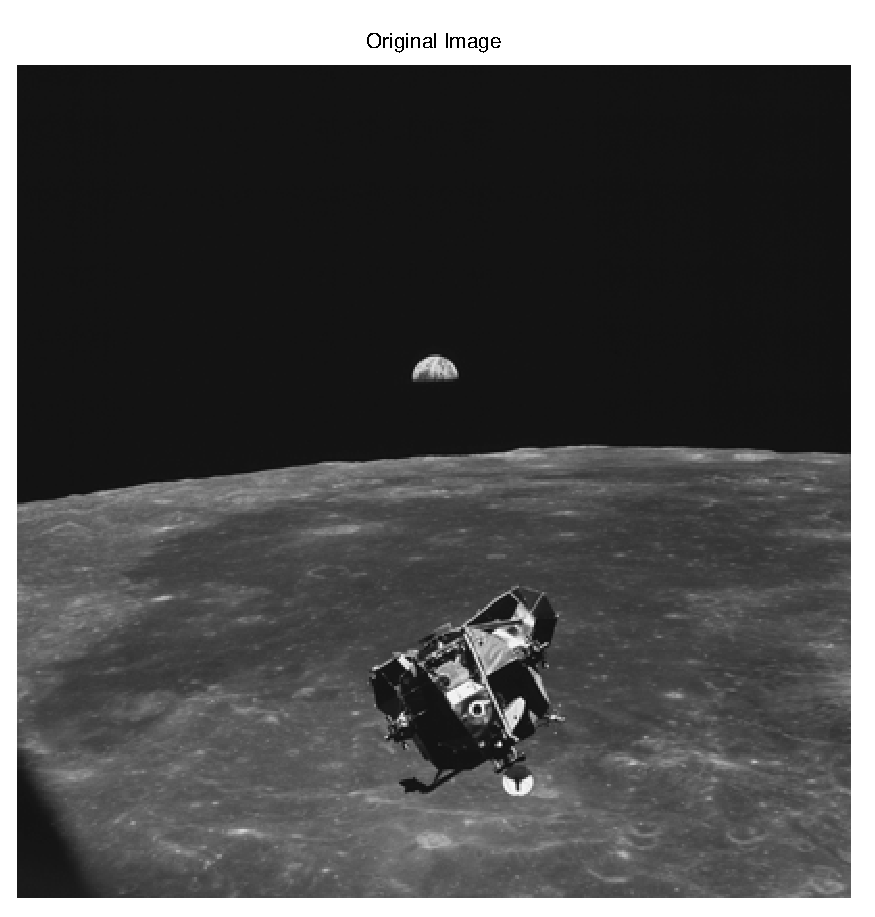
\includegraphics [width=4in]{hw4_01.eps}


\subsection*{Problem 1}

\begin{par}
An edge detection in the space domain.
\end{par} \vspace{1em}


\subsection*{Parts 1 and 2}

\begin{par}
Apply the horizontal and vertical sobel mask to the image. show the results.
\end{par} \vspace{1em}
\begin{verbatim}
figure('name', 'sobel masks using custom convultion')
subplot(121)

sobelX=double([-1 0 1; -2 0 2; -1 0 1])
horiz = convolution(I, sobelX);
imshow(im2uint8(horiz));
title('sobelX')

subplot(122)
sobelY=double([1 2 1; 0 0 0; -1 -2 -1])
vert = convolution(I, sobelY);
imshow(im2uint8(vert));
title('sobelY')
\end{verbatim}

        \color{lightgray} \begin{verbatim}
sobelX =

    -1     0     1
    -2     0     2
    -1     0     1


sobelY =

     1     2     1
     0     0     0
    -1    -2    -1

\end{verbatim} \color{black}
    
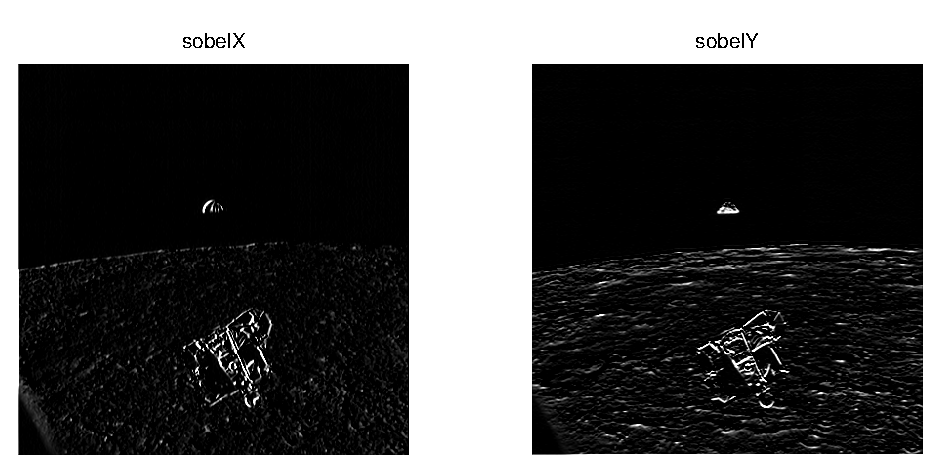
\includegraphics [width=4in]{hw4_02.eps}


\subsection*{Part 3}

\begin{par}
Use the magnitude to combine edges and show result
\end{par} \vspace{1em}
\begin{verbatim}
figure('name','magnitude'); %pop pop
magnitude = abs(horiz) + abs(vert);
imshow(magnitude);
title('approximation of magnitude');
\end{verbatim}

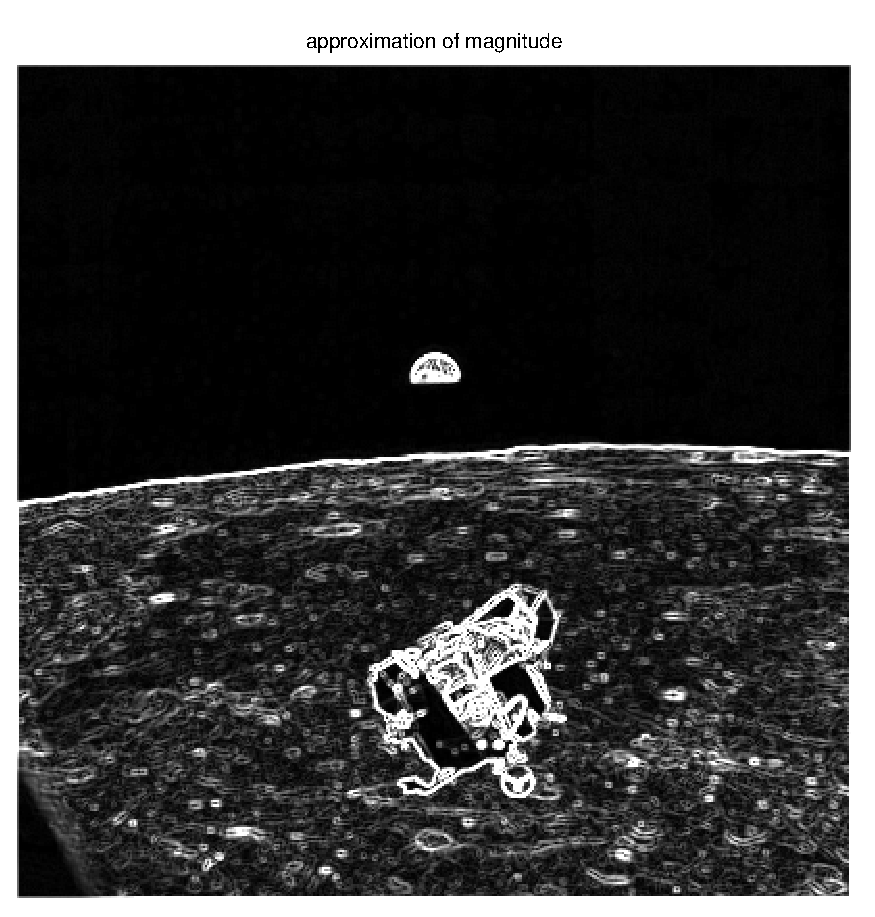
\includegraphics [width=4in]{hw4_03.eps}


\subsection*{Part 4}

\begin{par}
Use different constant for c in sobel mask. try different values and see what happens.
\end{par} \vspace{1em}
\begin{verbatim}
figure('name', 'various values for c in sobel mask')
subplot(221)
c=1;
sobelX=double([-1 0 1; -c 0 c; -1 0 1]);
sobelY=double([1 c 1; 0 0 0; -1 -c -1]);
h=convolution(I,sobelX);
v=convolution(I,sobelY);
C=(abs(h)+abs(v));
imshow(C);
title('c=1')

subplot(222);
c=3;
sobelX=double([-1 0 1; -c 0 c; -1 0 1]);
sobelY=double([1 c 1; 0 0 0; -1 -c -1]);
h=convolution(I,sobelX);
v=convolution(I,sobelY);
C=(abs(h)+abs(v));
imshow(C);
title('c=3')

subplot(223)
c=5;
sobelX=double([-1 0 1; -c 0 c; -1 0 1]);
sobelY=double([1 c 1; 0 0 0; -1 -c -1]);
h=convolution(I,sobelX);
v=convolution(I,sobelY);
C=(abs(h)+abs(v));
imshow(C);
title('c=5')


subplot(224)
c=10;
sobelX=double([-1 0 1; -c 0 c; -1 0 1]);
sobelY=double([1 c 1; 0 0 0; -1 -c -1]);
startS=tic; %asked for part 6
h=convolution(I,sobelX);
v=convolution(I,sobelY);
C=(abs(h)+abs(v));
sobeltime= toc(startS);
imshow(C);
title('c=10')
\end{verbatim}

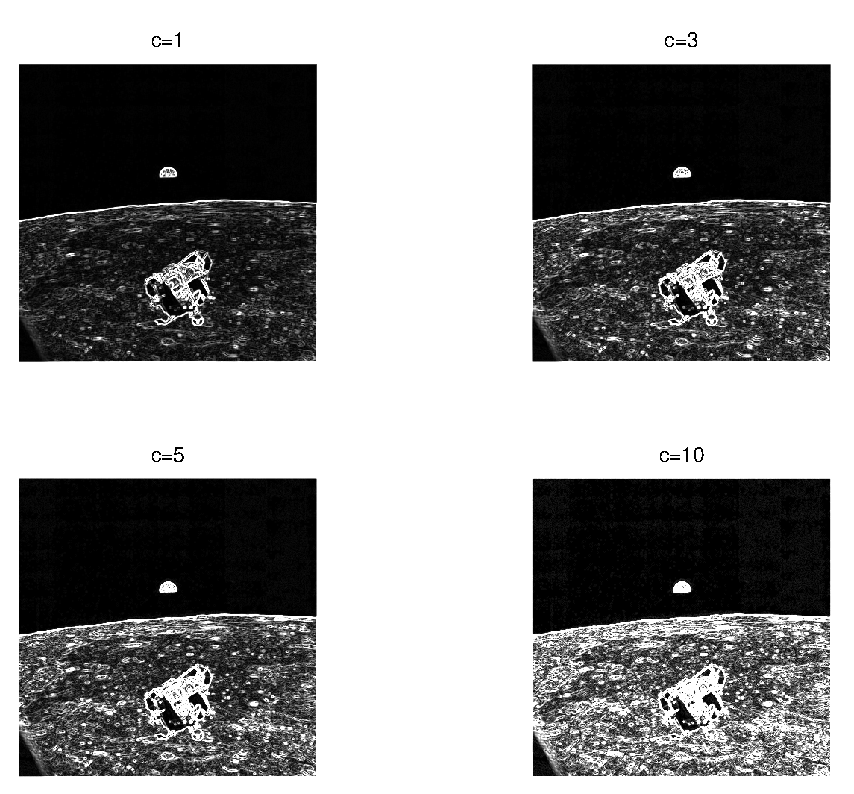
\includegraphics [width=4in]{hw4_04.eps}


\subsection*{Part 5}

\begin{par}
Use the Laplacian mask to edge detect same image, compare results.
\end{par} \vspace{1em}
\begin{verbatim}
figure('name', 'laplacian mask')
L=[0 1 0; 1 -4 1; 0 1 0];
startL = tic;
laplacedI=convolution(I,L);
laplacetime = toc(startL);
imshow(im2uint8(laplacedI)), title('laplacian mask');
rmpath ../commonFunctions
\end{verbatim}

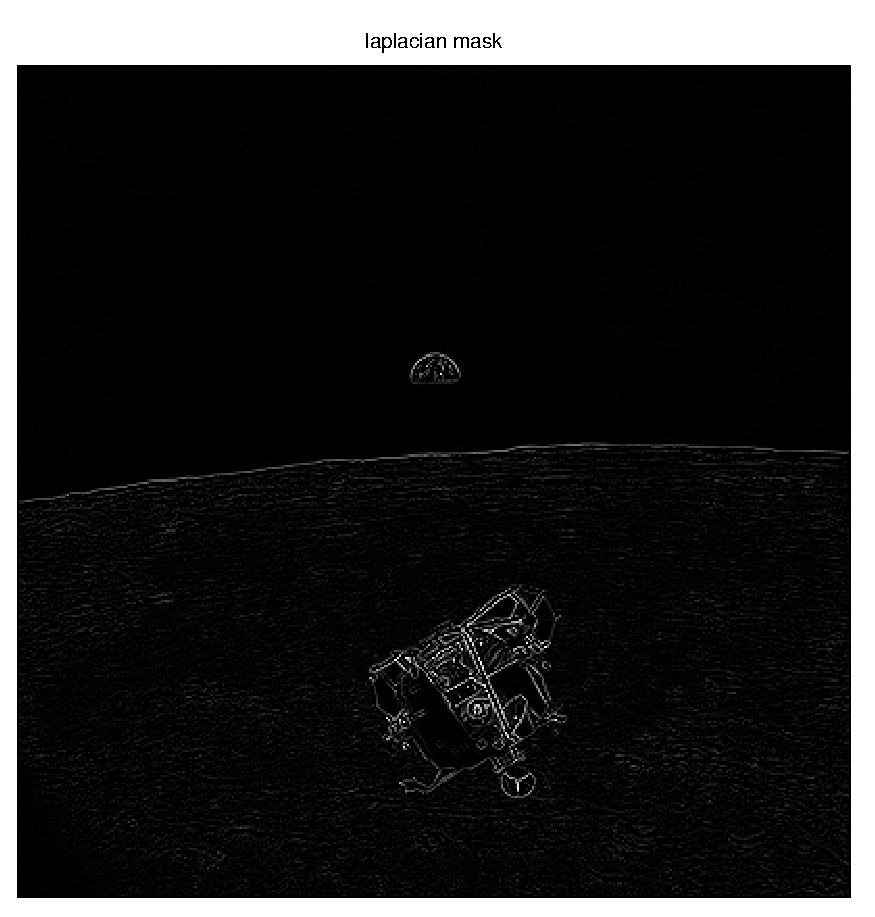
\includegraphics [width=4in]{hw4_05.eps}


\subsection*{Part 6}

\begin{par}
compare computation times
\end{par} \vspace{1em}
\begin{verbatim}
sprintf('sobel approach: %s',sobeltime)
sprintf('laplacian approach: %s', laplacetime)
\end{verbatim}

        \color{lightgray} \begin{verbatim}
ans =

sobel approach: 1.466107e-01


ans =

laplacian approach: 7.633747e-02

\end{verbatim} \color{black}
    

\subsection*{Problem 2}

\begin{par}
Edge detection in the frequency domain.
\end{par} \vspace{1em}


\subsection*{Part 1}

\begin{par}
Obtain the FFT of the horizontal and vertical Sobel masks. You need to perform zero padding.
\end{par} \vspace{1em}
\begin{verbatim}
addpath ../commonFunctions
I2 = getIMG('Soyuz_TMA-19_spacecraft_departs_the_ISS.jpg');
rmpath ../commonFunctions
I2 = im2double(rgb2gray(imresize(I2,[401,401])));
imshow(I2);

figure('name','ffts of sobel masks');
c=2;
sobelX=double([-1 0 1; -c 0 c; -1 0 1]);
sobelY=double([1 c 1; 0 0 0; -1 -c -1]);
%work on making this more general..........
sobelX1 = padarray(sobelX,[199,199]);
sobelFFTX=fft2(sobelX1);
%work on making this more general..........
sobelY1 = padarray(sobelY,[199,199]);
sobelFFTY=fft2(sobelY1);

subplot(121), imshow(sobelFFTX), title('sobelX fft');
subplot(122), imshow(sobelFFTY), title('sobelY fft');
\end{verbatim}

        \color{lightgray} \begin{verbatim}Warning: Displaying real part of complex input. 
Warning: Displaying real part of complex input. 
\end{verbatim} \color{black}
    
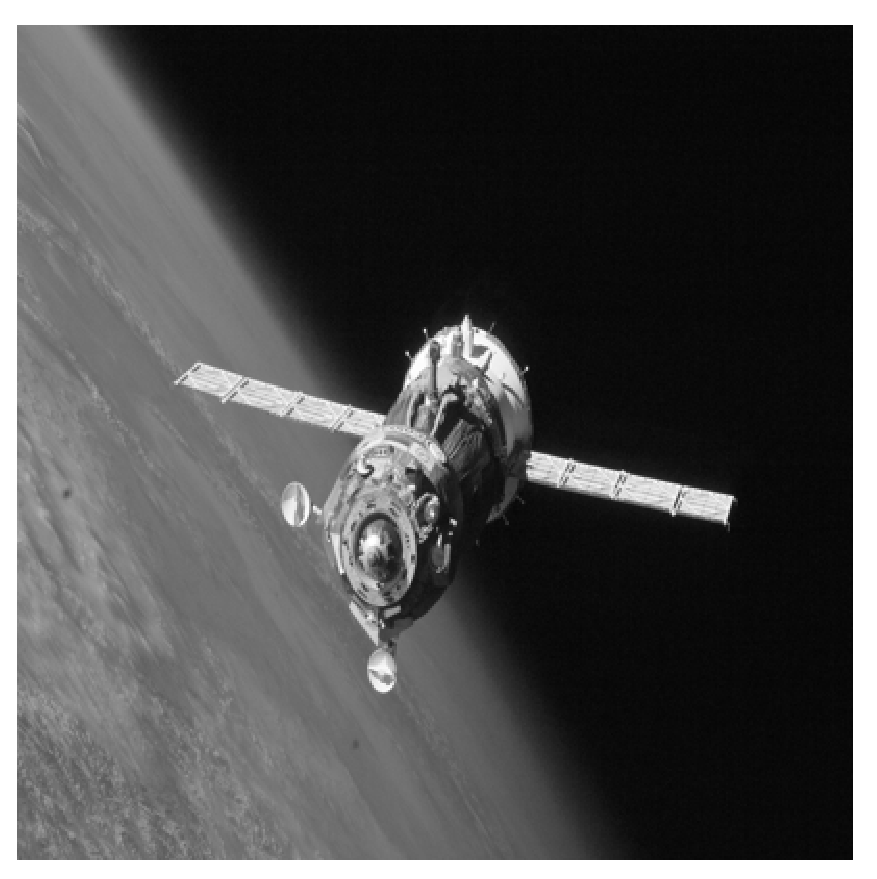
\includegraphics [width=4in]{hw4_06.eps}

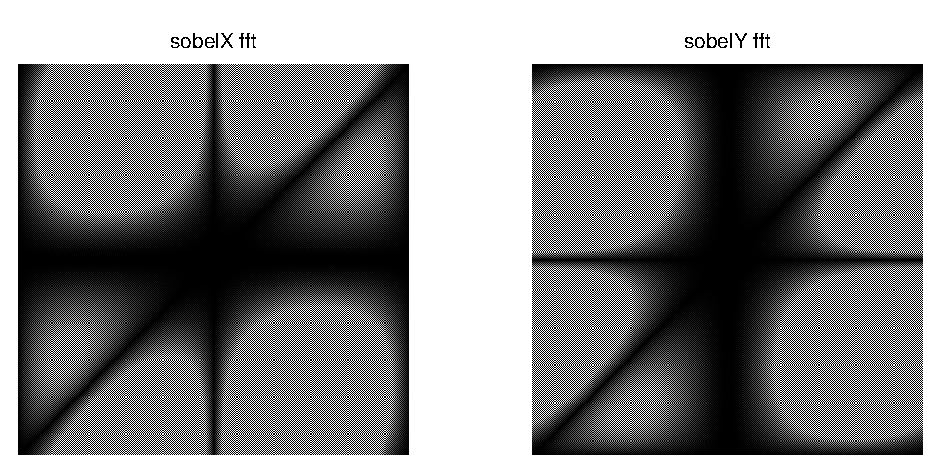
\includegraphics [width=4in]{hw4_07.eps}


\subsection*{Part 2}

\begin{par}
Perform filtering in the frequency domain using the horizontal Sobel mask
\end{par} \vspace{1em}
\begin{verbatim}
figure('name', 'frequency horizontal filtering');
horizF=fft2(I2).*sobelFFTX;
horizS=ifft2(horizF);
dmin = min(min(abs(horizS)));
dmax = max(max(abs(horizS)));
subplot(121), imshow(horizF), title('horizontal sobel freq');
subplot(122), imshow(ifftshift(horizS),[dmin dmax]), title('filtered img');
\end{verbatim}

        \color{lightgray} \begin{verbatim}Warning: Displaying real part of complex input. 
\end{verbatim} \color{black}
    
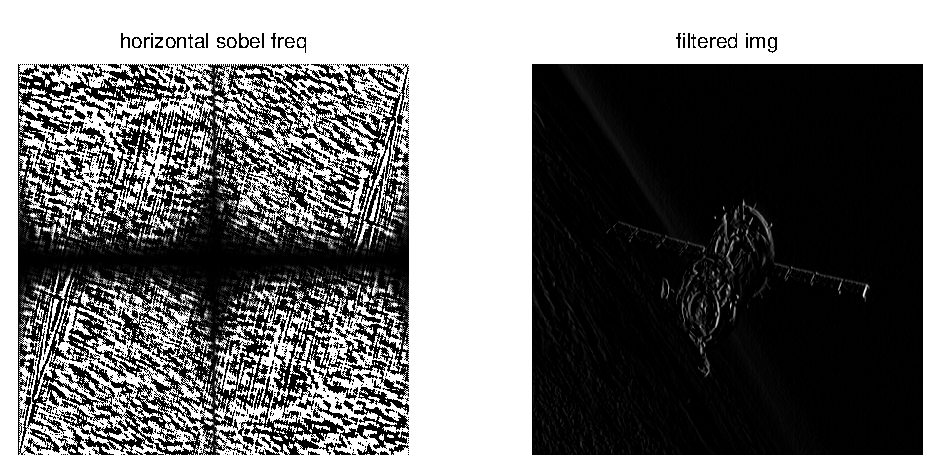
\includegraphics [width=4in]{hw4_08.eps}


\subsection*{Part 3}

\begin{par}
Perform filtering in the frequency domain using the vertical Sobel mask
\end{par} \vspace{1em}
\begin{verbatim}
figure('name', 'frequency vertical filtering');
vertF=fft2(I2).*sobelFFTY;
vertS=ifft2(vertF);
dmin = min(min(abs(vertS)));
dmax = max(max(abs(vertS)));
subplot(121), imshow(vertF), title('horizontal sobel freq');
subplot(122), imshow(ifftshift(vertS),[dmin dmax]), title('filtered img');
\end{verbatim}

        \color{lightgray} \begin{verbatim}Warning: Displaying real part of complex input. 
\end{verbatim} \color{black}
    
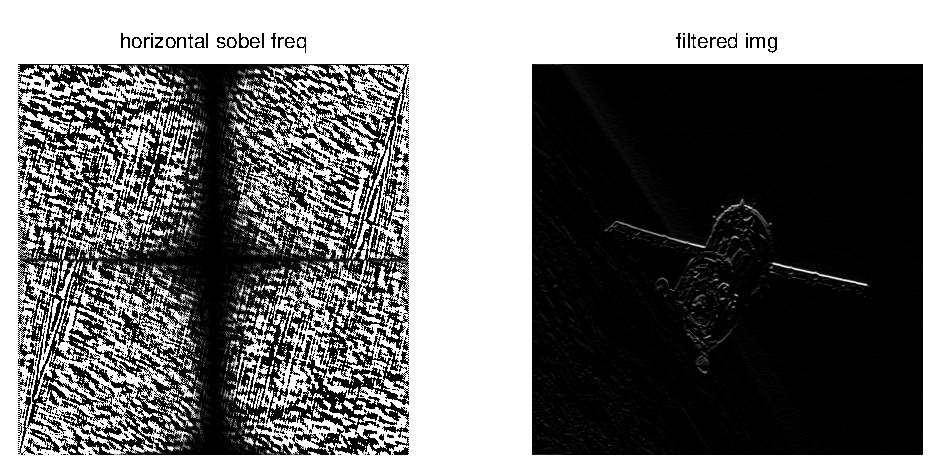
\includegraphics [width=4in]{hw4_09.eps}


\subsection*{Part 4}

\begin{par}
Obtain the FFT of the Laplacian mask. You need to perform zero padding.
\end{par} \vspace{1em}
\begin{verbatim}
L1 = fft2(padarray(L,[199,199]));
\end{verbatim}


\subsection*{Part 5}

\begin{par}
Perform filtering in the frequency domain using Laplacian to detect the edges.
\end{par} \vspace{1em}
\begin{verbatim}
figure('name','laplacian frequency filtering');
lapF=fft2(I2).*L1;
lapS=ifft2(lapF);
dmin = min(min(abs(lapS)));
dmax = max(max(abs(lapS)));
imshow(ifftshift(lapS),[dmin dmax]), title('Laplacian filtered img freq');
\end{verbatim}

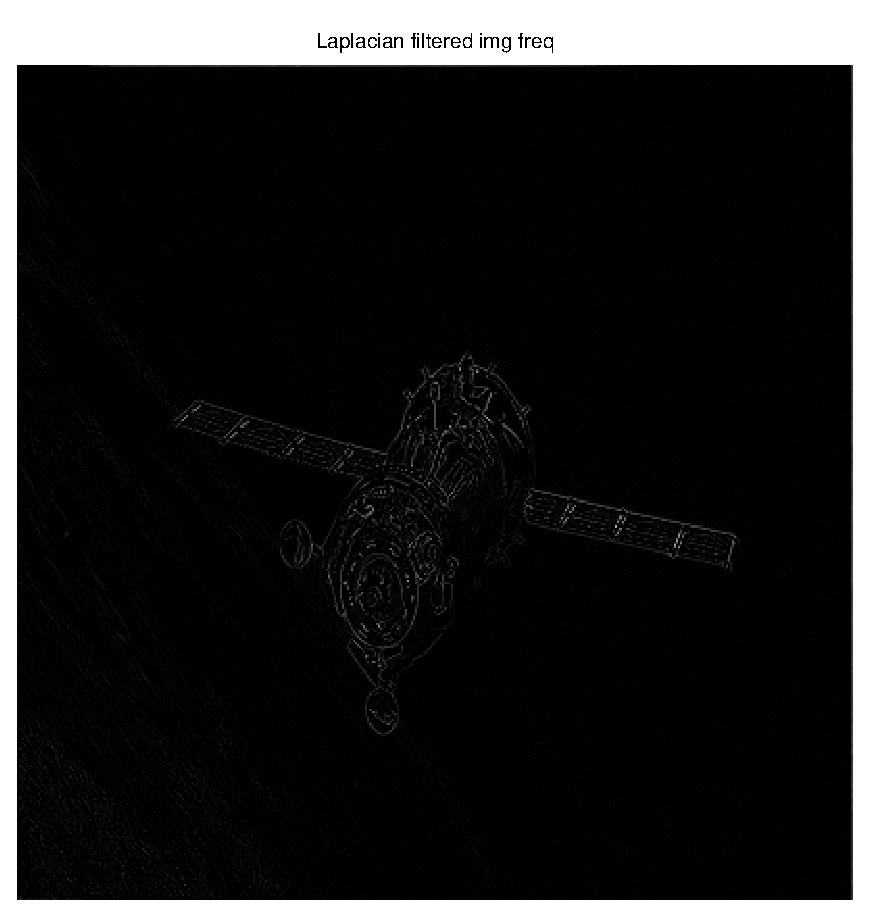
\includegraphics [width=4in]{hw4_10.eps}


\subsection*{Part 6}

\begin{par}
Construct a 3 by 3 mask for the Laplacian of Gaussian (LoG) and then obtain its FFT. You can use fspecial for this question
\end{par} \vspace{1em}
\begin{verbatim}
addpath ../commonFunctions
gauss=gaussfilter(3, 1/2);
LoG=L*gauss;
LoGF=fft2(LoG);
rmpath ../commonFunctions
%LoG=fspecial('log',[401,401]);
%LoGF=fft2(LoG);
\end{verbatim}


\subsection*{Parts 7 and 8}

\begin{par}
Perform filtering in the frequency domain using LoG to detect the edges
\end{par} \vspace{1em}
\begin{verbatim}
figure('name','laplacian of gaussian freq filtering');
I3=fft2(I2).*L1;
lapS=ifft2(I3);
dmin = min(min(abs(lapS)));
dmax = max(max(abs(lapS)));
imshow(ifftshift(lapS),[dmin dmax]);
title('Laplacian of gaussian filtered img freq');
\end{verbatim}

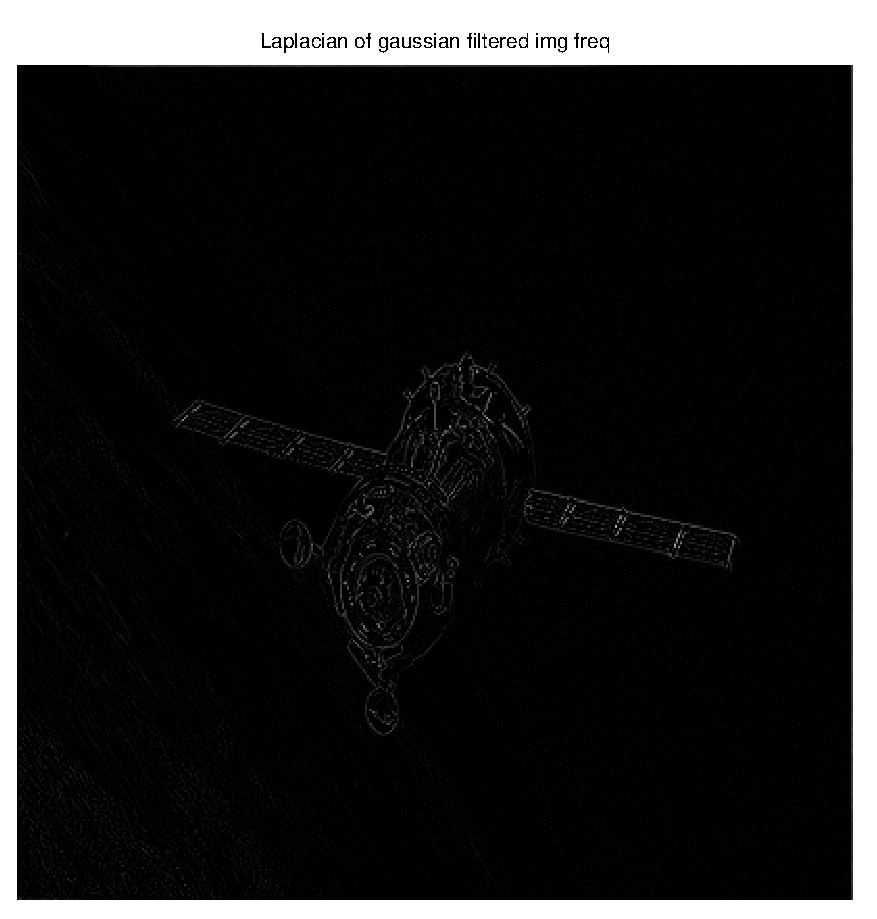
\includegraphics [width=4in]{hw4_11.eps}


\subsection*{Problem 3}

\begin{par}
The Harris detector was introduced in 1988 for corner detection. An illustration is shown in figure 2. Apply the Harris detector to an image of your choice. Pick an image with visible corners. Mark all corners on the image in a similar way to figure 2
\end{par} \vspace{1em}
\begin{verbatim}
figure('name','corner detection');
C=corner(I2); %to find corner points
imshow(I2);hold on, plot(C(:,1),C(:,2),'ro')
title('corners detected')
figure('name','corner detection2')
C=corner(I); %to find corner points
imshow(I);hold on, plot(C(:,1),C(:,2),'ro')
title('corners detected 2');
\end{verbatim}

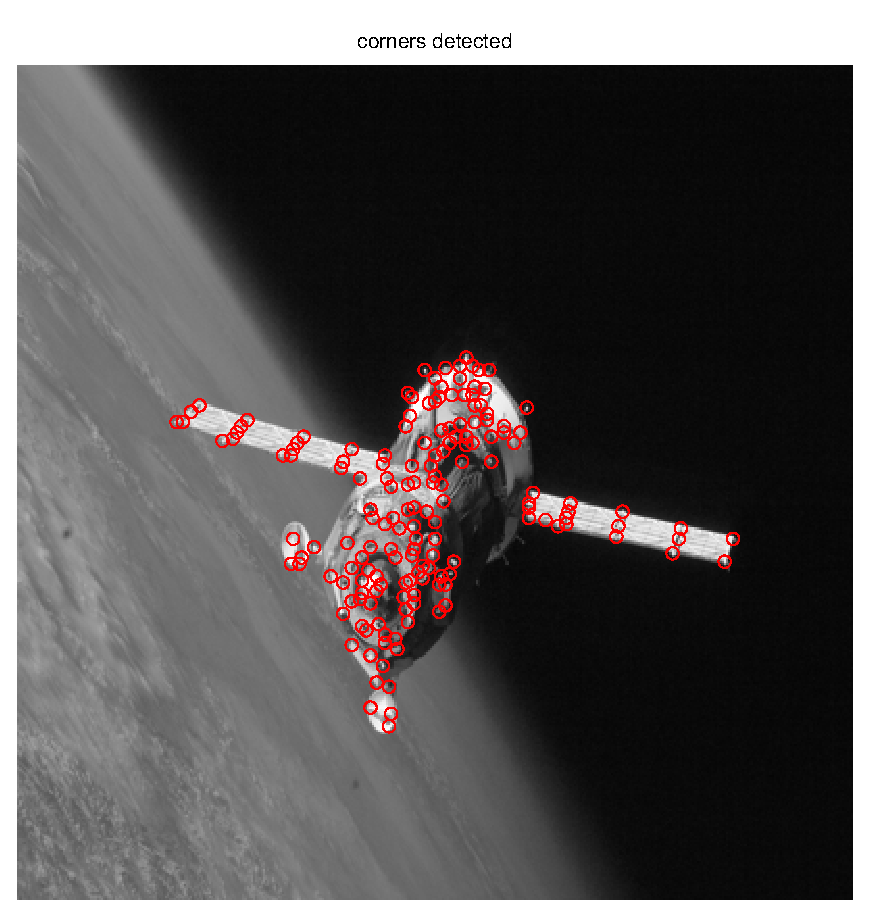
\includegraphics [width=4in]{hw4_12.eps}

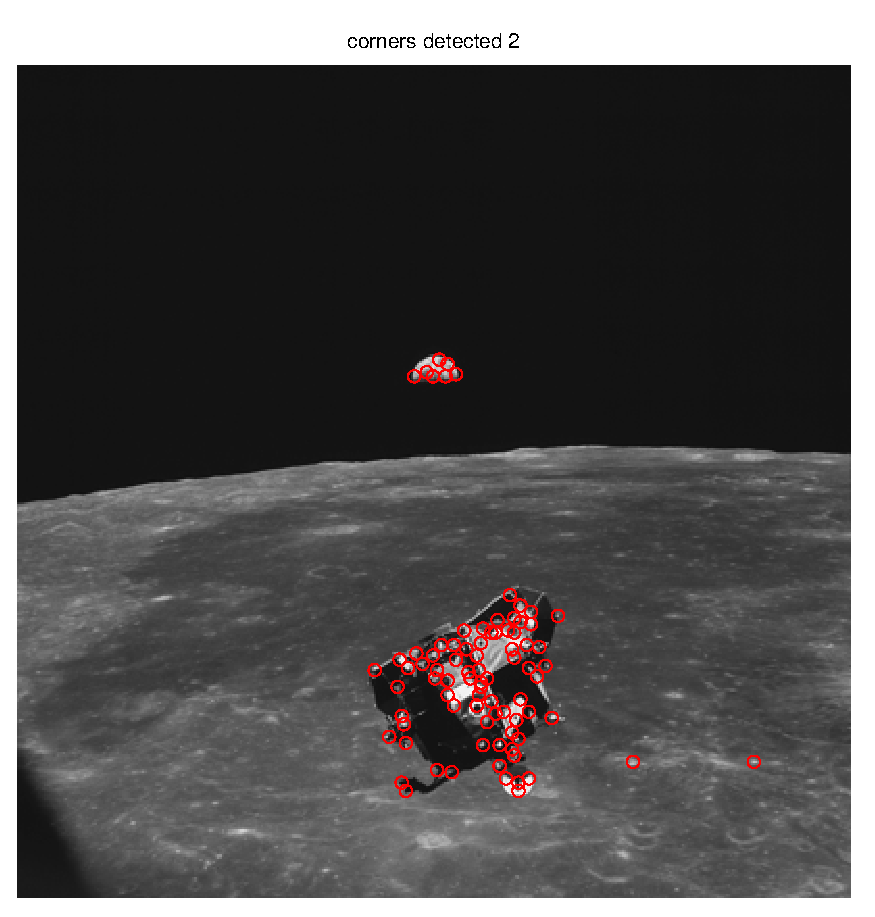
\includegraphics [width=4in]{hw4_13.eps}



\end{document}
    
